Our study cohort consisted of 52 patients with T2W, ADC, and B2000 MR images. For every patient we also had a prostate contour segmentation acquired using technique Ref. \citenum{cheng2014atlas} and tumor annotations done by an expert radiologist. Figure \ref{fig:Fig1} shows an example of the original image sequences and the regions of interest.     

 \begin{figure} [ht]
   \begin{center}
   \begin{tabular}{c}
   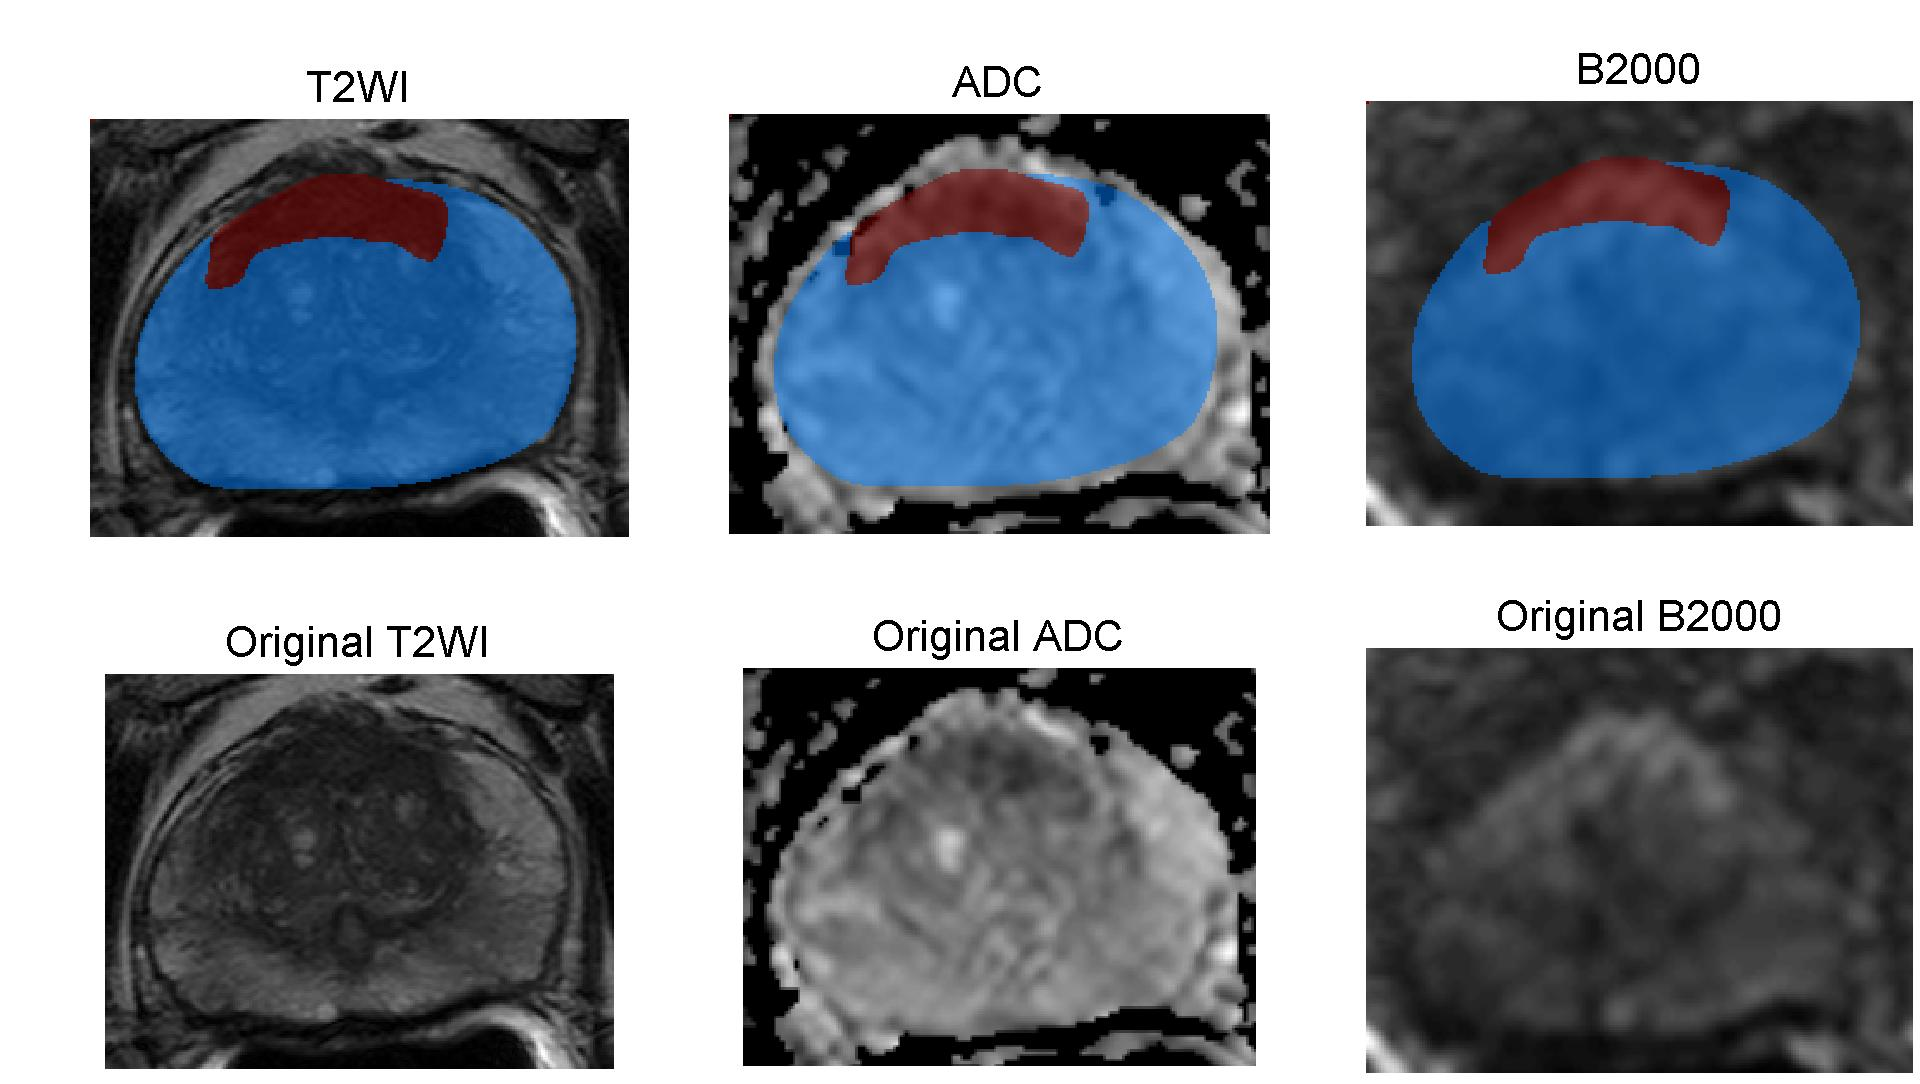
\includegraphics[height=5cm]{Figure1}
   \end{tabular}
   \end{center}
   \caption[Fig1]
   { \label{fig:Fig1} 
In the bottom row are the original T2W, ADC, and B2000 MR images, and the top row displays the tumor and prostate annotations overlaid on top of the original images.}
   \end{figure} 
   The patients in the study presented with lesions of various severity and location. Biopsy results are used to characterize the lesions. Table 1 has all the biopsy points for the study cohort stratified by zone (peripheral or transition) and Gleason score(6-9), where the higher the score the more severe the lesion. 

\begin{table}[ht]
\caption{Lesions stratified by location and severity} 
\label{tab:table1}
\begin{center}       
\begin{tabular}{|l|l|l|l|l|l|l|} 
\hline
\rule[-1ex]{0pt}{3.5ex} Zone &	Benign &	Gleason 6 &	Gleason 7 &	Gleason 8 &	Gleason 9 &	Total\\
\hline
\rule[-1ex]{0pt}{3.5ex} Peripheral &	24 &	5 &	19 &	10 &	3 &	61 \\
\rule[-1ex]{0pt}{3.5ex} Transition &	15 &	8 &	21 &	13 &	7 &	64 \\
\rule[-1ex]{0pt}{3.5ex} Overall &	39 &	13 &	40 &	23 &	10 &	125 \\ 
\hline
\end{tabular}
\end{center}
\end{table}


